%%%%%%%%%%%%%%%%%%%%%%%%%%%%%%%%%%%%%%%%%
% University/School Laboratory Report
% LaTeX Template
% Version 4.0 (March 21, 2022)
%
% This template originates from:
% https://www.LaTeXTemplates.com
%
% Authors:
% Vel (vel@latextemplates.com)
% Linux and Unix Users Group at Virginia Tech Wiki
%
% License:
% CC BY-NC-SA 4.0 (https://creativecommons.org/licenses/by-nc-sa/4.0/)
%
%%%%%%%%%%%%%%%%%%%%%%%%%%%%%%%%%%%%%%%%%

%----------------------------------------------------------------------------------------
%	PACKAGES AND DOCUMENT CONFIGURATIONS
%----------------------------------------------------------------------------------------

\documentclass[
	letterpaper, % Paper size, specify a4paper (A4) or letterpaper (US letter)
	10pt, % Default font size, specify 10pt, 11pt or 12pt
]{CSUniSchoolLabReport}

%----------------------------------------------------------------------------------------
%	REPORT INFORMATION
%----------------------------------------------------------------------------------------

\title{ECE 398-MA \\ Introduction to Modern Communication with Python and SDR \\ Python Lab 3} % Report title

\author{Noah Breit} % Author name(s), add additional authors like: '\& James \textsc{Smith}'

\date{\today} % Date of the report

%----------------------------------------------------------------------------------------

\begin{document}

\maketitle % Insert the title, author and date using the information specified above

% \begin{center}
% 	\begin{tabular}{l r}
% 		Date Performed: & February 13, 2022 \\ % Date the experiment was performed
% 		Partners: & Cecilia \textsc{Smith} \\ % Partner names
% 		& Tajel \textsc{Khumalo} \\
% 		Instructor: & Professor \textsc{Rivera} % Instructor/supervisor
% 	\end{tabular}
% \end{center}

% If you need to include an abstract, uncomment the lines below
%\begin{abstract}
%	Abstract text
%\end{abstract}

%----------------------------------------------------------------------------------------
%	OBJECTIVE
%----------------------------------------------------------------------------------------

\section{Assignment 1}

\begin{lstlisting}[language=Python]
	
import numpy as np
import matplotlib.pyplot as plt
from scipy.signal import hilbert

# Define simulation parameters
N = 1000    # Number of samples
fs = 100e3  # Sampling rate (Hz)
dt = 1/fs   # Sampling period
fc = 20e3    # Carrier frequency (Hz)
t = np.arange(N) / fs  # Time vector

# FM/PM Modulation Parameters
kf = 500  # Frequency deviation constant (for FM)
kp = np.pi / 2  # Phase deviation constant (for PM)

# Message signal (square wave)
message = np.concatenate([np.ones(N//2), -1*np.ones(N//2)])

############# YOUR CODE STARTS HERE #############
# FM Modulation (integrate message signal)
fm_signal = np.cos(2 * np.pi * fc * t + 2 * np.pi * kf * np.cumsum(message) * dt)

# PM Modulation (direct phase shift)
pm_signal = np.cos(2 * np.pi * fc * t + kp * message)
############# YOUR CODE ENDS HERE #############

# Plot results
plt.figure()
plt.subplot(3, 1, 1)
plt.plot(t, message, label='Message')
plt.xlabel("Time [s]")
plt.ylabel("Amplitude")
plt.legend()

plt.subplot(3, 1, 2)
plt.plot(t, fm_signal, label='FM')
plt.xlabel("Time [s]")
plt.ylabel("Amplitude")
plt.legend()

plt.subplot(3, 1, 3)
plt.plot(t, pm_signal, label='PM')
plt.xlabel("Time [s]")
plt.ylabel("Amplitude")
plt.legend()
plt.tight_layout()
plt.savefig("assignment1a.png")
plt.show()

import numpy as np
import matplotlib.pyplot as plt

# Define simulation parameters
N = 1000    # Number of samples
fs = 100e3  # Sampling rate (Hz)
dt = 1/fs   # Sampling period
fc = 20e3   # Carrier frequency (Hz)
t = np.arange(N) / fs  # Time vector

# FM/PM Modulation Parameters
kf = 500  # Frequency deviation constant (for FM)
kp = np.pi / 2  # Phase deviation constant (for PM)

# Original Message Signal (square wave)
original_message = np.concatenate([np.ones(N//2), -1*np.ones(N//2)])

# Modified Message Signal (integral of the original square wave)
modified_message = np.cumsum(original_message) * dt

# FM Modulation (integrate original message signal)
integrated_message = np.cumsum(original_message) * dt
fm_signal = np.cos(2 * np.pi * fc * t + 2 * np.pi * kf * integrated_message)

# PM Modulation (use modified message signal)
pm_signal = np.cos(2 * np.pi * fc * t + kp * modified_message)

# Plot results
plt.figure()
plt.subplot(3, 1, 1)
plt.plot(t, modified_message, label='Modified Message')
plt.xlabel("Time [s]")
plt.ylabel("Amplitude")
plt.legend()

plt.subplot(3, 1, 2)
plt.plot(t, fm_signal, label='FM')
plt.xlabel("Time [s]")
plt.ylabel("Amplitude")
plt.legend()

plt.subplot(3, 1, 3)
plt.plot(t, pm_signal, label='PM')
plt.xlabel("Time [s]")
plt.ylabel("Amplitude")
plt.legend()
plt.tight_layout()
plt.savefig('assignment1b.png')
plt.show()

\end{lstlisting}

\begin{figure}[H] % [H] forces the figure to be placed exactly where it appears in the text
	\centering % Horizontally center the figure
	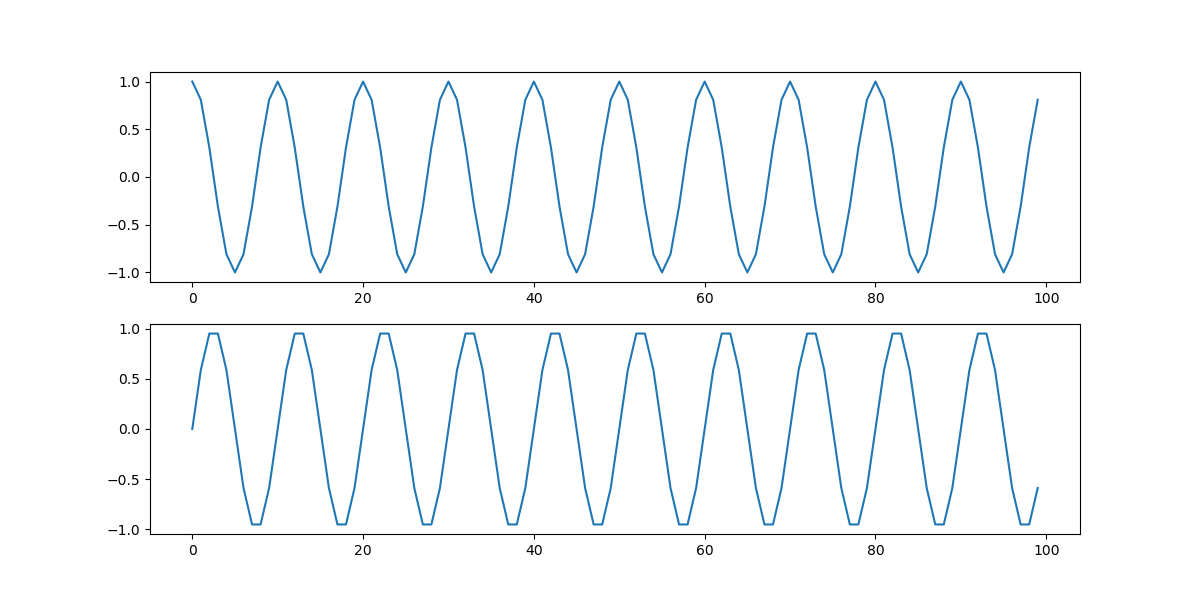
\includegraphics[width=1.2\textwidth]{assignment1.png} % Include the figure
	\caption{Unmodified FM and PM Signals}
	\label{fig:block}
\end{figure}

\begin{figure}[H] % [H] forces the figure to be placed exactly where it appears in the text
	\centering % Horizontally center the figure
	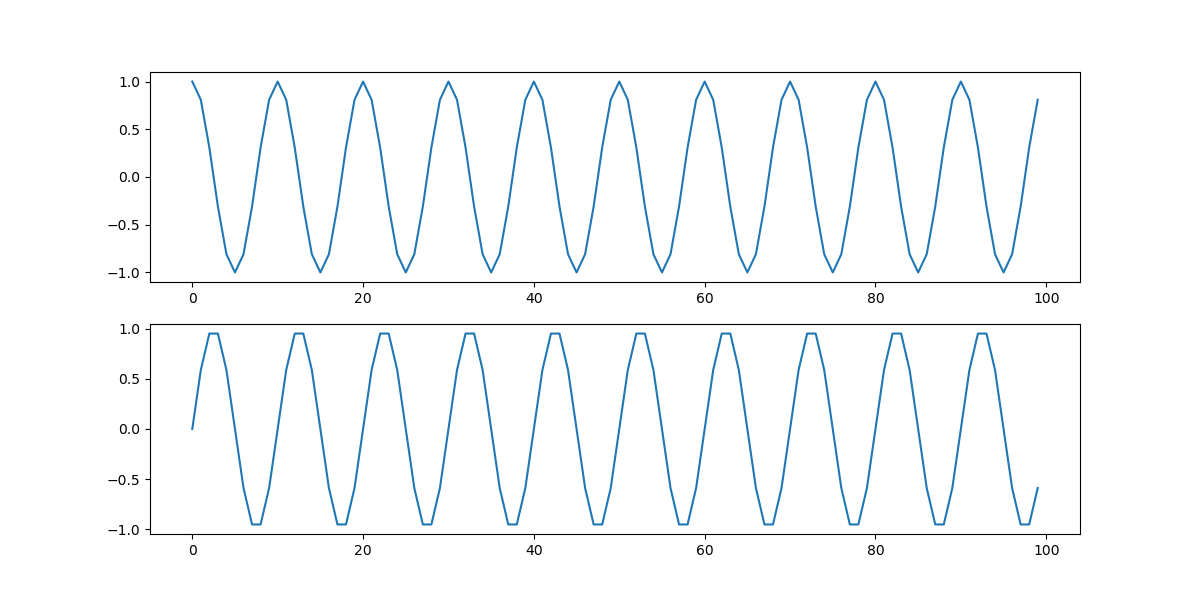
\includegraphics[width=1.2\textwidth]{assignment1.png} % Include the figure
	\caption{Modified FM and PM Signals}
	\label{fig:block}
\end{figure}

\section{Assignment 2}


\begin{lstlisting}[language=Python]
	

\end{lstlisting}

\begin{figure}[H] % [H] forces the figure to be placed exactly where it appears in the text
	\centering % Horizontally center the figure
	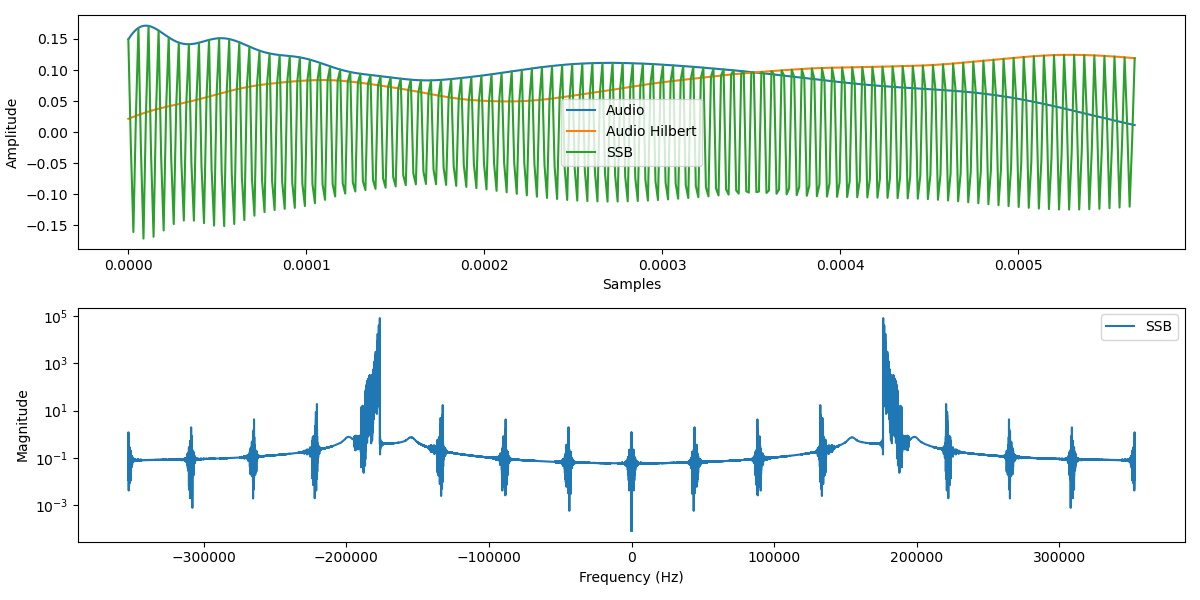
\includegraphics[width=1.2\textwidth]{assignment2a.png} % Include the figure
	\caption{Upper Side Band (USSB) of Audio Signal}
	\label{fig:block}
\end{figure}

\begin{figure}[H] % [H] forces the figure to be placed exactly where it appears in the text
	\centering % Horizontally center the figure
	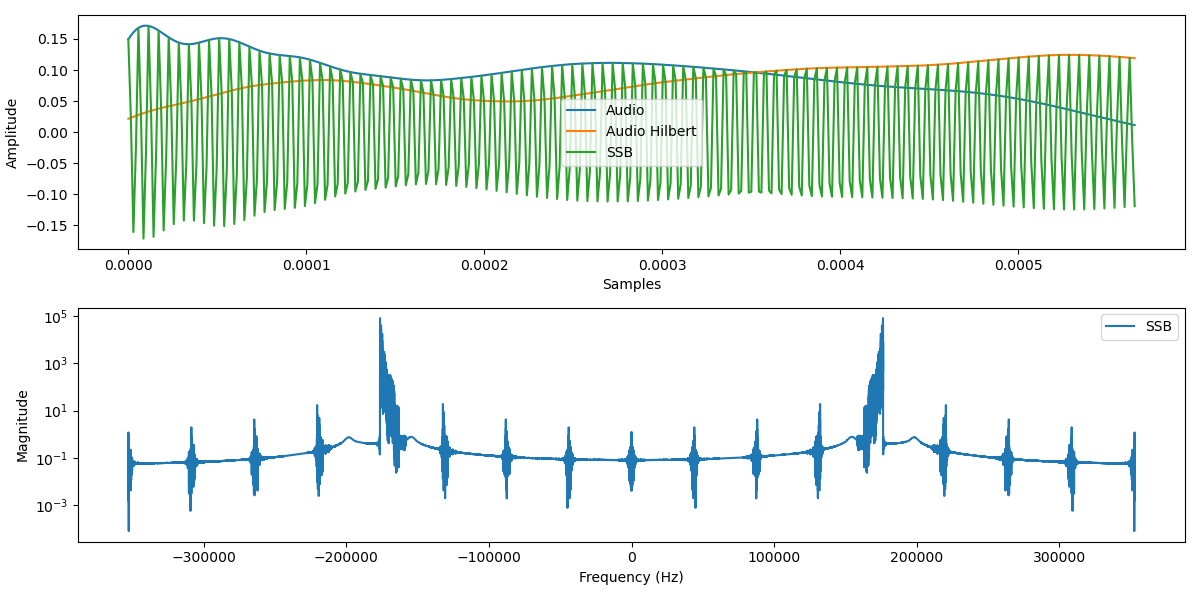
\includegraphics[width=1.2\textwidth]{assignment2b.png} % Include the figure
	\caption{Lower Side Band (LSSB) of Audio Signal}
	\label{fig:block}
\end{figure}

\section{Assignment 3}

\begin{lstlisting}[language=Python]
	

\end{lstlisting}

\begin{figure}[H] % [H] forces the figure to be placed exactly where it appears in the text
	\centering % Horizontally center the figure
	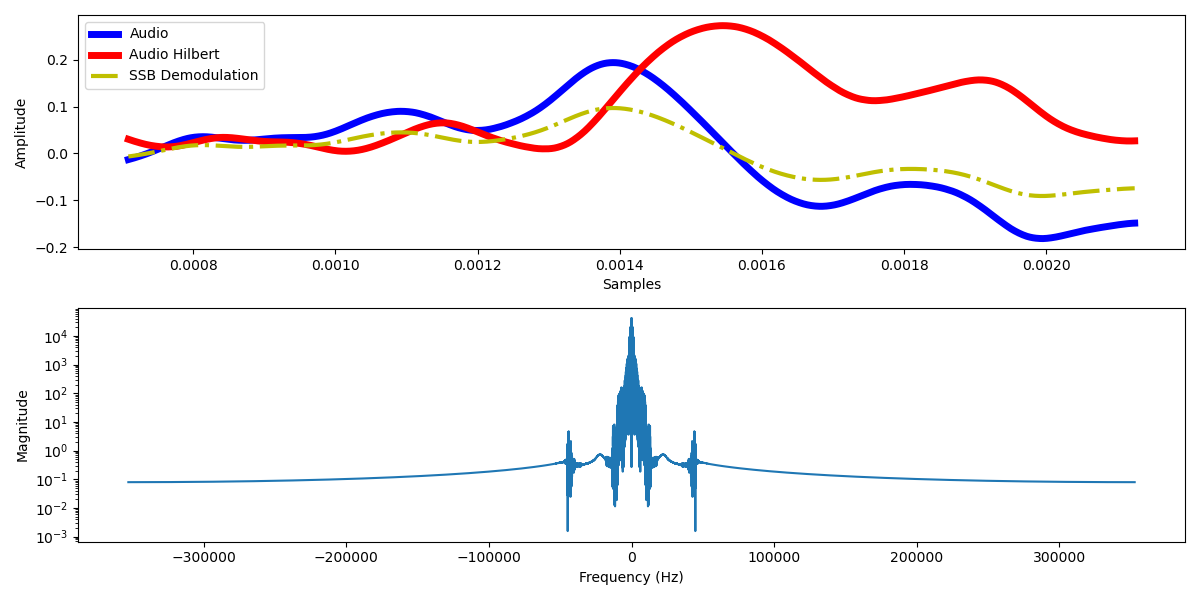
\includegraphics[width=1.2\textwidth]{assignment3.png} % Include the figure
	\caption{Demodulated Audio Signal: No Phase Offset}
	\label{fig:block}
\end{figure}

\begin{figure}[H] % [H] forces the figure to be placed exactly where it appears in the text
	\centering % Horizontally center the figure
	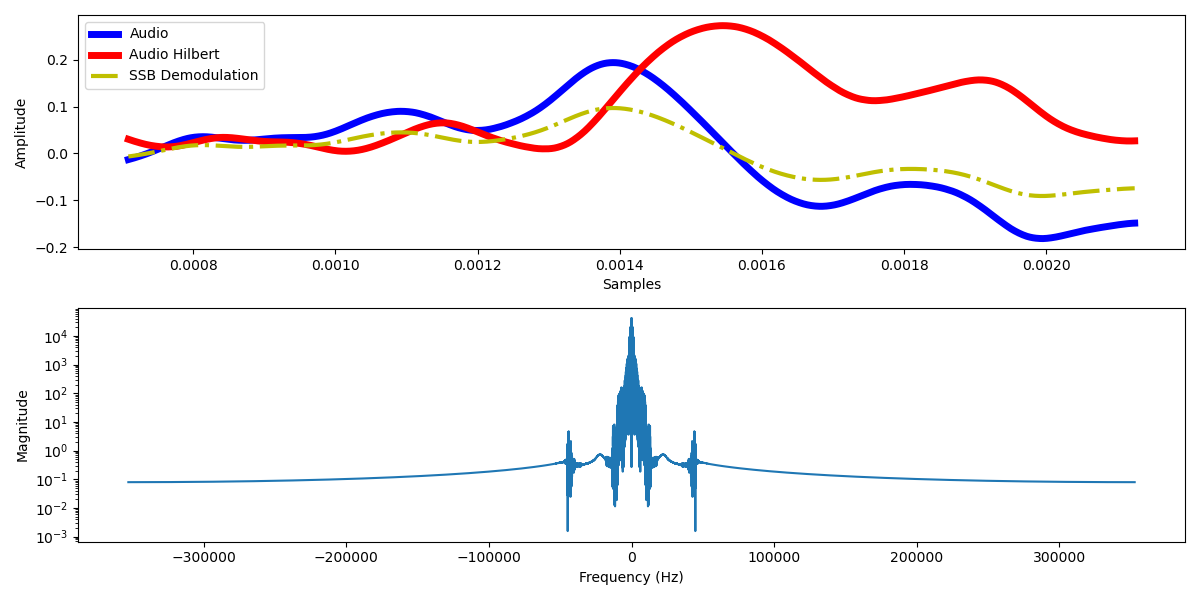
\includegraphics[width=1.2\textwidth]{assignment3b.png} % Include the figure
	\caption{Demodulated Audio Signal: Phase Offset of pi/2}
	\label{fig:block}
\end{figure}

\begin{figure}[H] % [H] forces the figure to be placed exactly where it appears in the text
	\centering % Horizontally center the figure
	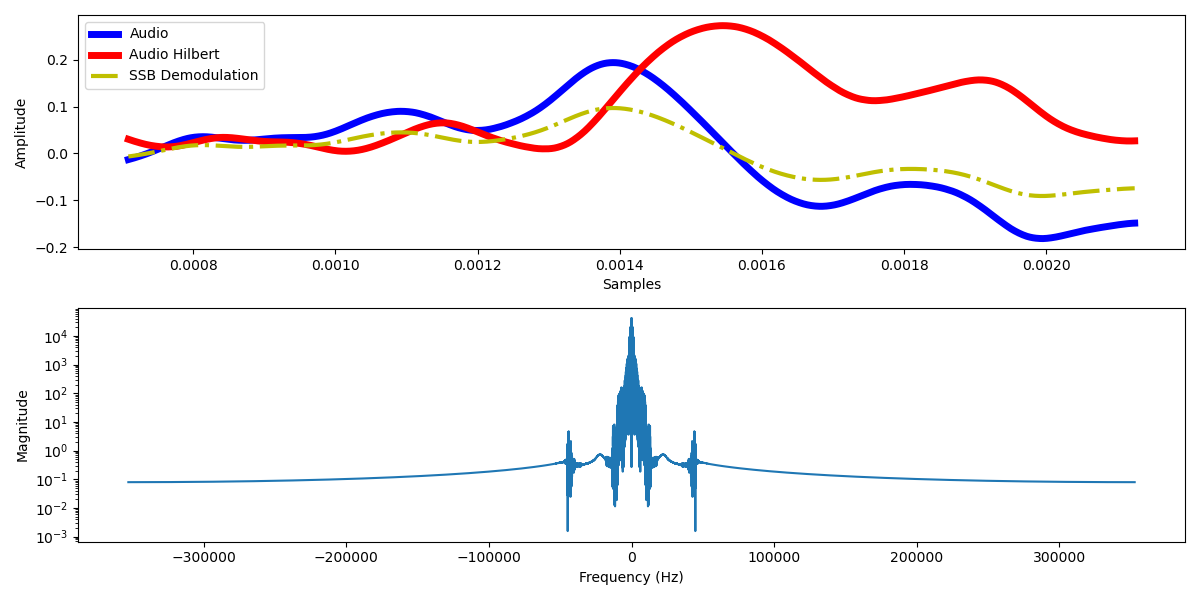
\includegraphics[width=1.2\textwidth]{assignment3c.png} % Include the figure
	\caption{Demodulated Audio Signal: Phase Offset of pi/4}
	\label{fig:block}
\end{figure}

\end{document}